\chapter{Computer Vision}

In questo capitolo vorrei fare un discorso generale riguardo la computer vision,
mi piacerebbe dare un taglio cognitivo al discorso ovvero vorrei discutere di come
l'ispezione ottica richieda strumenti matematici e informatici volti ad emulare
la comprensione, mi piacerebbe anche evidenziare come la telecamera sia da considereare
un sensore tramite cui è apprezzata la realtà.

\section{Ispezione automatica piuttosto che manuale}

qui vorrei parlare delle esigenze risolte dalla visione computerizzata in caso di
ispezioni ottiche, quali sono gli obiettivi e le sfide, ripetibilità, oggettivizzazione,
accuratezza.

\section{Luce}

\'{E} ampiamente riconosciuto che l'appropriatezza della luce e la qualità della stessa
siano aspetti critici nella creazione di un sistema di visione pronto e robusto.
Progettare un ambiente di analisi robusto massimizzerà la riuscita del progetto in termini
di tempo, sforzo e risorse impiegate.

Storicamente, la luce è stato sempre l'ultimo aspetto ad essere specificato, sviluppato o finaziato, questo tipo di approccio derivava principalmente dall'assenza di prodotti commerciali espressamente rivolti alla machine vision, ciò portava all'adozioni di prodotti consumer quali lampade a incandescenza e/o fluorescenza.

Ciò che è realmente richiesto per la realizzazione di sistemi di ispezione industriale è il controllo dell' illuminazione volto a produrre:

\begin{itemize}
	\item Illuminazione appropriata dei campioni da analizzare;
	\item Standardizzazione delle componenti, tecniche, implementazioni e dell'utilizzo del sistema di illuminazione;
	\item Riproducibilità dei risultati delle ispezioni;
	\item Robustezza delle ispezioni a variazioni dell'ambiente di ispezione;
\end{itemize} 

per ottenere risultati consistenti nel design di un sistema di illuminazione bisognerebbe tenere a mente i punti di seguito riassunti:

\begin{itemize}
	\item Tipologie di luce e vantaggi e svantaggi nell'applicazione;
	\item Efficienza quantica del sensore e range spettrale;
	\item Tecniche di illuminazione e campi di applicazione relativi alla tipologia di superficie da ispezionare;
	\item Requisiti e limitazioni di ciascuna tecnica di illuminazione;
	\item Geometria della luce;
	\item Struttura (Pattern) della luce;
	\item Lunghezza d'onda della luce;
	\item Filtraggio della luce;
	\item Analisi dettagliata dell'ambiente da illuminare (requisiti e vincoli);
	\item Raccolta di campioni e verifica delle interazioni con le varie tecniche di illuminazione;
\end{itemize}

\subsection{Caratteristiche della luce}

La luce è una radiazione elettromagnetica visibile all'occhio umano e responsabile del senso della vista,
la luce visibile è di solito definita avente lunghezza d'onda compresa tra i 500nm e i 700 nm, compresa tra gli infrarossi aventi lunghezze d'onda maggiori e gli ultra violetti aventi lunghezze d'onda inferiori.

Le proprietà primarie della luce sono l'intensità, la direzione di propagazione, la frequenza (o lunghezza d'onda) e la polarizzazone.

La luce viene emessa in piccoli pacchetti detti fotoni che esibiscono proprietà duali sia di particella che onda.

Il comportamento di un onda elettromagnetica dipende dalla sua lunghezza d'onda, quando essa colpiscce singoli atomi o molecole il suo comportamento dipende da quanta energia ogni singolo pacchetto trasporta.

\subsection{Rifrazione - legge di Snell}

\begin{figure}
\centering
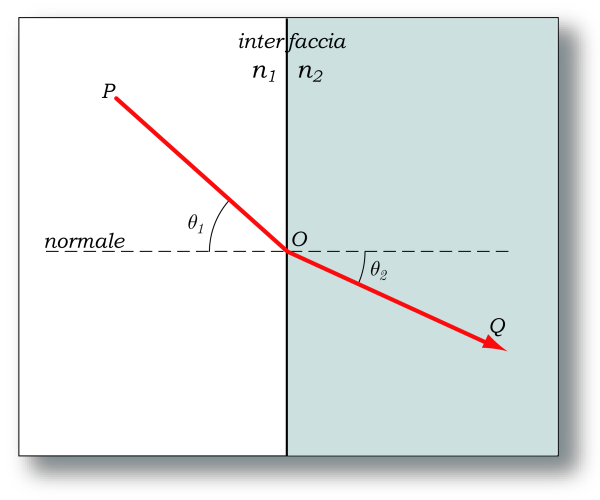
\includegraphics[width=.5\textwidth]{img/Legge_di_Snell.png}
\caption{Rifrazione}\label{fig:snell}
\end{figure}

La rifrazione è la deviazione subita da un'onda che ha luogo quando questa passa da un mezzo ad un altro 
nel quale la sua velocità di propagazione cambia.
La legge di Snell, nota anche come legge di Descartes o legge di Snell-Descartes (o legge di Cartesio o legge di Snell-Cartesio), descrive le modalità di rifrazione di un raggio luminoso nella transizione tra due mezzi con indice di rifrazione diverso, e deriva dall'equazione iconale.
La figura \ref{fig:snell} mostra due mezzi trasmissivi con indice di rifrazione $n_1$ (a sinistra) e $n_2$ (a destra) in contatto tra loro attraverso una superficie, che viene chiamata interfaccia (linea verticale in figura). Nel caso $n_2 > n_1$, la luce ha una velocità di fase più bassa nel secondo mezzo.
Il raggio luminoso $PO$ proveniente dal mezzo di sinistra colpisce l'interfaccia nel punto $O$. A partire da tale punto O tracciamo una retta perpendicolare all'interfaccia stessa, che viene chiamata normale all'interfaccia (linea orizzontale in figura). L'angolo tra la normale e il raggio luminoso $PO$ viene chiamato angolo d'incidenza, $\theta_1$.
Il raggio attraversa l'interfaccia e prosegue nel mezzo di destra, indicato come $OQ$. L'angolo che tale raggio (rifratto) forma con la normale si chiama angolo di rifrazione, $\theta_2$.
La legge di Snell fornisce la relazione tra gli angoli $\theta_1$ e $\theta_2$:
\[n_1 \sin(\theta_1)=n_2 \sin(\theta_2)\]
Si noti che nel caso $\theta_1 = 0\degree$ (ovvero il raggio risulta perpendicolare all'interfaccia) la soluzione è $\theta_2 = 0\degree$ per qualunque valore di $n_1$ e $n_2$. In altri termini, un raggio che entra in un mezzo in modo perpendicolare alla sua superficie non viene mai deviato.
Quanto detto sopra vale anche nel caso di un raggio luminoso che passa da un mezzo più denso a uno meno denso; la simmetria della legge di Snell mostra che gli stessi percorsi luminosi sono validi anche nella direzione opposta.
Una regola di carattere qualitativo per determinare la direzione della rifrazione è che il raggio luminoso è sempre più vicino alla normale dal lato del mezzo più denso.
La legge di Snell è valida in generale solo per mezzi isotropi, come il vetro. Nel caso di mezzi anisotropi (ad esempio alcuni cristalli) il fenomeno della birifrangenza può dividere in due il raggio rifratto. Si vengono allora ad avere due raggi, uno ordinario (raggio o) che segue la legge di Snell, e uno straordinario (raggio e) che può non essere complanare con quello incidente.

\subsection{Riflessione}


La riflessione è il fenomeno per cui un'onda, che si propaga lungo l'interfaccia tra differenti mezzi, cambia di direzione a causa di un impatto con un materiale riflettente.
Assorbimento, riflessione e trasmissione sono i fenomeni che avvengono quando la luce interagisce con la materia. Quando l'energia radiante incide su un corpo, una parte viene assorbita, una parte viene riflessa e una parte viene trasmessa. Per la legge di conservazione dell'energia, la somma delle quantità di energia rispettivamente assorbita, riflessa e trasmessa è uguale alla quantità di energia incidente.
Per indicare il tipo di riflessione di cui si tratta si usano gli aggettivi:
\begin{itemize}
\item Spettrale: per indicare la radiazione monocromatica, cioè considerata lunghezza d'onda per lunghezza d'onda;
\item Radiante (contrapposto a luminosa): per indicare che la radiazione è data in termini di energia totale, cioè è espressa mediante grandezze radiometriche;
\item Luminosa (contrapposto a radiante): per indicare che la radiazione è pesata secondo la funzione di efficienza luminosa dell'occhio, cioè è espressa in grandezze fotometriche;
\end{itemize}


\begin{figure}[!h]
\centering
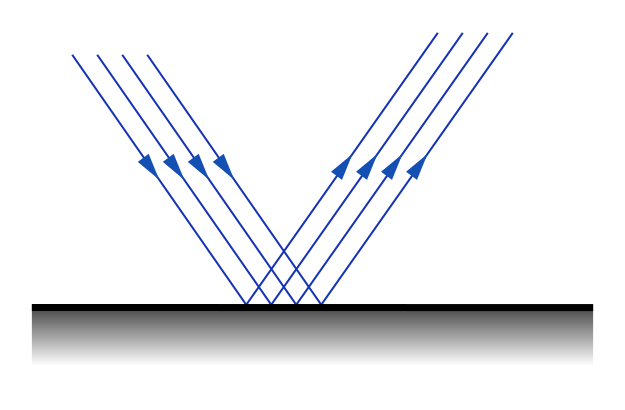
\includegraphics[width=.5\textwidth]{img/riflessione.png}
\caption{Riflessione Speculare}\label{fig:riflessione1}
\end{figure}


\begin{figure}[!h]
\centering
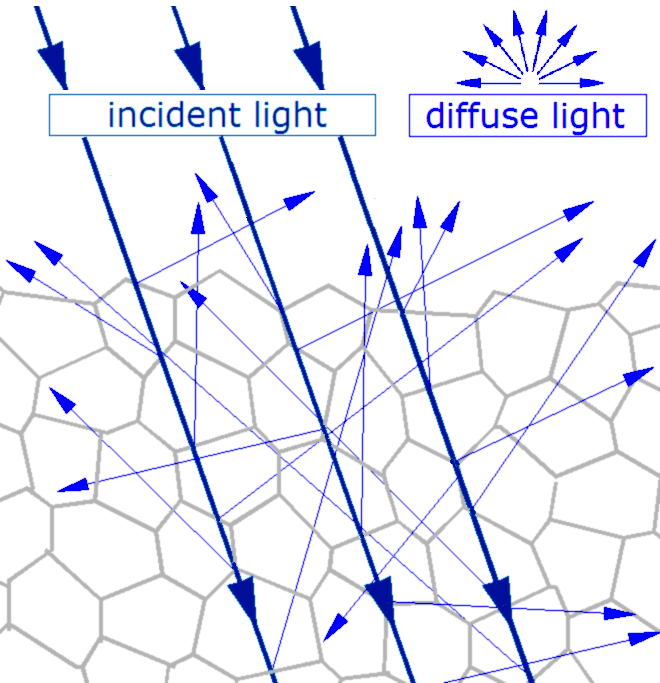
\includegraphics[width=.5\textwidth]{img/riflessione_diffusa.png}
\caption{Riflessione Diffusa}\label{fig:riflessione2}
\end{figure}

La riflessione può avvenire:
\begin{itemize}
\item Specularmente (riflessione speculare o regolare) cioè in una unica (o quasi) direzione
\item Diffusamente (riflessione diffusa) cioè in varie direzioni;
\end{itemize}
La riflettanza (reflectance) è il rapporto tra flusso riflesso e flusso incidente valutato per ogni lunghezza d'onda. Essendo definita come rapporto di grandezze omogenee, la riflettanza è una grandezza adimensionale e viene espressa in percentuale (0-100\%) o come fattore (0.0-1.0). Inoltre riguarda il flusso e quindi la totalità della radiazione riflessa nella emisfera.
La riflettanza non è solo funzione della lunghezza d'onda ma anche dell'illuminazione, della geometria di irradiamento e della geometria di visione (cioè della geometria con cui si illumina il corpo e della geometria con cui si misura la quantità riflessa), per cui è necessario definire una grandezza più generale della riflettanza, cioè il fattore di riflessione.
Si fa riferimento al diffusore riflettente ideale. Si tratta di un corpo (ideale, cioè teorico) che non assorbe e non trasmette, ma riflette diffusamente la radiazione ricevuta con radianza o luminanza uguale per ogni angolo di riflessione e indipendentemente dalla direzione della radiazione incidente. Come prima applicazione del concetto di diffusore riflettente ideale si definisce il fattore di radianza (radiance factor) o il fattore di luminanza (luminance factor) come il rapporto tra la radianza di un'area e quella del diffusore ideale riflettente irradiato nello stesso modo.
Con riferimento a questo corpo ideale, il fattore di riflessione (reflectance factor o reflection factor) di un corpo è il rapporto tra il flusso riflesso dal corpo in un dato cono il cui vertice è sul corpo considerato e il flusso riflesso dal diffusore riflettente ideale.
Il fattore di riflessione è dunque una grandezza generica che corrisponde:
alla riflettanza spettrale se il cono è una emisfera;
al fattore di radianza spettrale se il cono è stretto.
Un tipico spettrofotometro è in grado di misurare il fattore di riflessione spettrale ad intervalli di 10 nm nell'intervallo da 380 a 730 nm.
La riflessione di onde elettromagnetiche è regolata da due leggi fondamentali, ricavabili dal principio di Fermat e dal principio di Huygens-Fresnel:

\begin{itemize}
\item Il raggio incidente, il raggio riflesso e la normale al piano nel punto di incidenza giacciono sullo stesso piano;
\item L'angolo di incidenza e l'angolo di riflessione sono uguali;
\end{itemize}

Un'onda elettromagnetica riflessa può subire uno sfasamento. Questo dipende dagli indici di rifrazione del mezzo nel quale viaggia la luce ($n1$) e del mezzo oltre la superficie riflettente ($n2$):

\begin{tabular}{l}
se $n1>n2$ non c'è sfasamento;\\
se $n1<n2$ la radiazione riflessa è sfasata di $\pi$, cioè di mezza lunghezza d'onda.\\
\end{tabular}

\subsection{Illuminazione direzionale}

Un illuminatore direzionale è costituito da una o più 
sorgenti di luce puntiforme che proiettano luce direzionale 
sulla parte da ispezionare, utilizzando questa tipologia di 
illuminatore è possibile ispezionare superfici piane non 
riflettenti poichè la luce raggiunge il sensore in maniera 
consistente. 

\subsection{Illuminazione tangenziale}

Un illuminatore tangenziale è costituito da una o più 
sorgente di luce direzionale aventi un elevato angolo di 
incidenza rispetto alla parte da ispezionare, ciò li rende 
adatti ad evidenziare difetti superficiali dell’oggetto che 
appaiono evidenziati sull’immagine.  
Tale metodologia e applicata con successo all’ispezione di 
componenti marcati con tecnologia DPM ( Direct Part 
Marking ) laser poichè la superficie incisa risulta evidenziata 
da questo tipo di illuminatore 

\subsection{Illuminazione diffusa}
Un illuminatore tangenziale è costituito da sorgente di luce 
diffusa ed estesa ciò li rende adatti nell’ispezione di parti 
che potrebbero creare riflessi illuminando in maniera 
omogenea e consistente l’area di ispezione, sono tuttav ia 
di difficile impiego in contesti dove gli ingombri sono 
ridotti per via delle grandi dimensioni ( Una sorgente di 
luce diffusa viene realizzata posizionando sorgenti di luce 
puntiforme lontano dall’area di ispezione )  
 
\subsection{illuminazione anulare}
Un illuminatore anulare è costituito da più sorgenti di luce 
puntiformi disposte coassialmente al dispositivo di 
imaging, ciò li rende adatti ad un ispezione simile a quelle 
possibili per mezzo di luce diffusa ma ne limita l’area 
ispezionata e la distanza di esercizio, tale tipologia di 
illuminazione produce inoltre fastidiosi riflessi circolari 
(rumore) 
 
\subsection{illuminazione diffusa assiale}
Un illuminatore diffuso assiale  è costituito da una 
sorgente di luce puntiforme direzionale orientata 
perpendicolarmente all’oggetto da ispezionare, tale luce 
colpisce un beam splitter riflettendosi prima sulla parte da 
ispezionare e poi sul dispositivo di imagin, ciò crea una 
luce diffusa senza riflessi circolari ma gli  ingombri di 
questi sistemi e la distanza di esercizio limitata ne 
vincolano l’utilizzo 

 


\section{Sensori}

questa sezione dovrebbe descrivere le varie tecnologie disponibili per la realizzazione di
sensori ottici utilizzati nelle odierne telecamere per applicazioni industriali.

\section{Algoritmi}
Qui vorrei discutere di alcuni algoritmi e tecniche importanti per il processamento delle immagini
e fare un parallelo con l'analisi dei segnali.

\subsection{Image Processing}
Qui vorrei parlare di tecniche generiche per il processamento delle immagini quali fitltraggio, filtraggio
morfologico, binarizzazione ecc.

\subsection{Object detection and recognition}	
Qui vorrei parlare di tecniche per object detection e recognition introducendo machine learning.

\endinput